\documentclass[10pt]{article}
\usepackage[utf8]{inputenc}
\usepackage[activeacute,spanish]{babel}
\usepackage[left=1.5cm,top=1.5cm,right=1.5cm, bottom=1.5cm,letterpaper, includeheadfoot]{geometry}

\usepackage{amssymb, amsmath, amsthm}
\usepackage{graphicx}
\usepackage{hyperref}
\usepackage{lmodern,url}
\usepackage{paralist} %util para listas compactas
\usepackage{xcolor}
\usepackage{bbm}
\usepackage{mathrsfs}
\usepackage{bbm}

%========PAQUETES AGREGADOS===========
%Pseudocodigo
\usepackage{pseudocode}
\usepackage[portuguese, boxruled]{algorithm2e}
\usepackage{wrapfig}
\usepackage{multicol}
\usepackage{graphicx}
\usepackage{caption}
\usepackage{subcaption}
%\captionsetup[table]{labelformat=empty}
\captionsetup[subfigure]{labelformat=empty}
\usepackage{cancel}
\usepackage{tikz}
\def\checkmark{\tikz\fill[scale=0.4](0,.35) -- (.25,0) -- (1,.7) -- (.25,.15) -- cycle;} 
%====================================

\usepackage{fancyhdr}
\pagestyle{fancy}
\fancypagestyle{plain}{%
\fancyhf{}
\lhead{\footnotesize\itshape\bfseries\rightmark}
\rhead{\footnotesize\itshape\bfseries\leftmark}
}


% macros
\newcommand{\Q}{\mathbb Q}
\newcommand{\R}{\mathbb R}
\newcommand{\N}{\mathbb N}
\newcommand{\Z}{\mathbb Z}
\newcommand{\C}{\mathbb C}
\newcommand{\BigO}{\mathcal{O}}
%Teoremas, Lemas, etc.
\theoremstyle{plain}
\newtheorem{teo}{Teorema}
\newtheorem{lem}{Lema}
\newtheorem{prop}{Proposición}
\newtheorem{cor}{Corolario}
\newtheorem{obs}{Observación}
\newtheorem{ej}{Ejemplo}
\renewcommand{\qedsymbol}{\rule{0.7em}{0.7em}}
\renewenvironment{proof}{{\bfseries \noindent Demostración}}{ \qed \\}


\theoremstyle{definition}
\newtheorem{defi}{Definición}
% fin macros


\newcommand{\catnum}{14} %numero de catedra
\newcommand{\fecha}{13 de Septiembre 2016 }

%%%%%%%%%%%%%%%%%%

%Macros para este documento
\newcommand{\cin}{\operatorname{cint}}



\begin{document}
%Encabezado
\fancyhead[L]{Facultad de Ciencias Físicas y Matemáticas}
\fancyhead[R]{Universidad de Chile}
\vspace*{-1.2 cm}
\begin{minipage}{0.6\textwidth}
\begin{flushleft}
\hspace*{-0.5cm}\textbf{MA3402-1 Estadística. Primavera 2016}\\
\hspace*{-0.5cm}\textbf{Profesor:} Raul Gouet\\
\hspace*{-0.5cm}\textbf{Escriba:} Manuel Cáceres\\
\hspace*{-0.5cm}\textbf{Fecha:} \fecha
\end{flushleft}
\end{minipage}
\begin{minipage}{0.36\textwidth}
\begin{flushright}

\includegraphics[scale=0.3]{imagenes/fcfm_dcc}
\end{flushright}
\end{minipage}
\bigskip
%Fin encabezado

\begin{center}
\LARGE\textbf{Clase \catnum}
\end{center}
\section{Paradigma Bayesiano de la Inferencia Estadística}
El origen de esta manera de abordar estos problemas de inferencia se debe (esencialmente) a Bayes y Laplace. El parámetro $\theta$ se comienza a considerar como una variable aleatoria también.
\section{Elementos de la inferencia Bayesiana}
\begin{enumerate}
\item Supongamos que $X$ tiene densidad $f(X|\theta)$ con $\theta \in \Theta$, parámetro en $\mathbb{R}^k$ y escribimos $f(X|\theta)$ para indicar que pensamos en la densidad condicional en $\theta$. Cambiamos la notación $f_{\theta}(X)$ por $f(X|\theta)$.
\item Disponemos de una densidad de probabilidad $\pi(\theta)$ sobre $\Theta$, llamémosla, densidad a priori. Esta densidad refleja nuestro conocimiento (o incertidumbre) sobre $\theta$.\\
\end{enumerate}
Con estos elementos se definen algunas distribuciones o probabilidades sobre espacios como $\mathfrak{X}\times\Theta,\mathfrak{X}$ o sobre $\Theta$.\\
La clave de estos cálculos es la fórmula de Bayes.\\
Caso elemental $(\Omega,\mathcal{F}, \mathbb{P}), A, B \subseteq \Omega$ con $\mathbb{P}(A), \mathbb{P}(B) >0$
\begin{align*}
\mathbb{P}(A|B) &= \frac{\mathbb{P}(A\cap B}{\mathbb{P}(B)}&\text{ (prob. condicional)}\\
\mathbb{P}(B|A) &= \frac{\mathbb{P}(A|B)\mathbb{P}(B)}{\mathbb{P}(A)} & \text{ (Bayes)}
\end{align*}
Si $\{B_{i}\}_{i\in I}$ una partición numerable de $\Omega$ con $\mathbb{P}(B_{i})>0$, entonces
\begin{align*}
\mathbb{P}(A) &= \sum_{i \in I}\mathbb{P}(A|B_{i}\mathbb{P}(B_{i})&\text{ (prob. condicional)}\\
\mathbb{P}(B_{i}|A) &= \frac{\mathbb{P}(A|B_{i})\mathbb{P}(B_{i})}{\sum_{i\in I}\mathbb{P}(A|B_{i})\mathbb{P}(B_{i})} & \text{ (Bayes)}
\end{align*}
También funciona con densidades (módulo que no se anula)\\
Si $(X,Y)$ tiene densidad $f_{X,Y}(x,y)$ y marginales $f_{X}, f_{Y}$ podemos definir $f_{X|Y}(x|y) = f_{X,Y}(x,y)/f_{Y}(y)$
\begin{align*}
\Rightarrow & f_{Y|X}(y|x) = \frac{f_{X|Y}(x|y)f_{Y}(y)}{\int f_{X|Y}(x|y)f_{Y}(y) dy}
\end{align*}
Par especificar un modelo bayesiano, debemos precisar $f(x|\theta), \Theta\ y\ \pi(\theta)$.\\
En la estadística bayesiana se manejan algunos principios axiomáticos a los que deben obedecer los procedimientos que utilicemos. En resumen, hay dos grandes principios:
\begin{enumerate}
\item \underline{Principio de suficiencia:} Toda inferencia sobre $\theta$ debe depender únicamente de un estadístico suficiente.
\item \underline{Principio de la verosimilitud:} Toda inferencia sobre $\theta$ debe basarse en la función de verosimilitud $f(X|\theta)$.
\end{enumerate}
Veamos densidades que se obtienen a partir de $f(X|\theta)$, considerada condicional de $X$ dado $\theta$ y $\pi(\theta)$, la densidad a priori:
\begin{enumerate}
\item $f(X,\theta) = f(X|\theta)\pi(\theta)$ la conjunta de $X,\theta$
\item $f(X) = \int f(X|\theta)\pi(\theta)d\theta$ la marginal
\item $\pi(\theta|X) = \frac{f(X|\theta)\pi(\theta)}{f(X)} = \frac{f(X|\theta)\pi(\theta)}{\int f(X|\theta)\pi(\theta)d\theta}$ la densidad a priori
\end{enumerate}
Frecuentemente se usa la notación $\pi(\theta|X) \underbrace{\alpha}_{\text{símbolo de proporcionalidad, puede depender de X}} f(X|\theta)\pi(\theta)$\\

Un problema del reverendo Bayes. Se echa a correr una bola en el intervalo [0,1], hasta que se detiene, en un punto P, que podemos considerar uniforme en [0,1]. Luego lanzamos suficientes bolitas de la misma manera y contamos el número $X$ de aquellas que se detienen antes de P.
\begin{center}
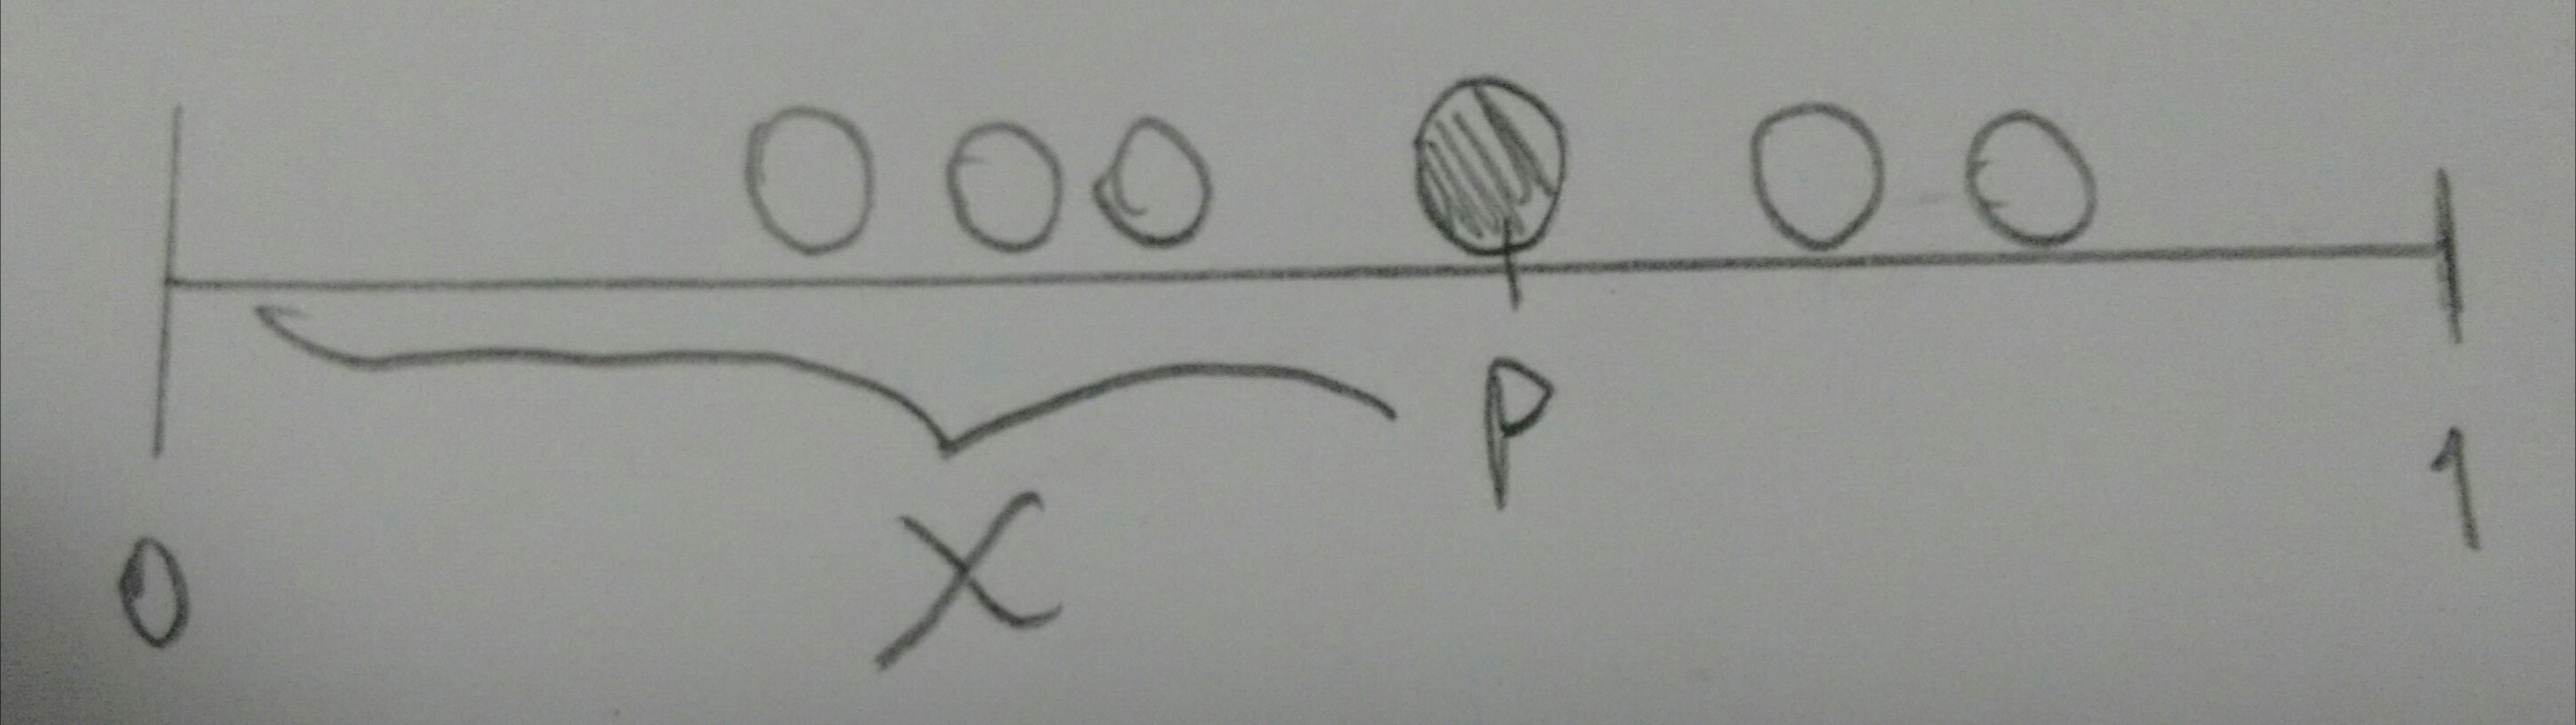
\includegraphics[scale=0.1]{imagenes/bayesiano1.jpg}
\end{center}
conociendo $X$, se puede decir algo sobre P. Es claro que $X$ condicional en P es Binomial(n,P) y que $\frac{X}{n}$ será una buena aproximación de P, aunque P es aleatorio.
\begin{align*}
\mathbb{E}(X|n|P) = P & \mathbb{E}()\\
\mathbb{E}(X|n) = \int_{0}^{1} p dp = \frac{1}{2}
\end{align*}
\begin{ej}
Consideremos el lanzamiento de una moneda con probabilidad $\theta \in [0,1] = \Theta$ desconocida, es decir, tenemos el clásico modelo de Bernoulli:
\begin{align*}
f(X|\theta) = \theta^{\sum X_{i}}(1-\theta)^{n-\sum X_{i}}\\
\theta\in \Theta, X = (X_{1},\ldots,X_{n}) \in \{0,1\}^n = \mathfrak{X}
\end{align*}
Supongamos que no sabemos nada sobre el parámetro, pero estamos obligados a entregar $\pi(\theta)$. Parece razonable postular $\pi(\theta)=c, \forall \theta\in\Theta$.\\
Como $\int_{0}^{1}\pi(\theta)d\theta = 1 \Rightarrow c = 1$
\begin{align*}
f(X,\theta) &= \theta^{\sum X_{i}} (1-\theta)^{n-\sum X_{i}} \mathbbm{1}_{[0,1]}(\theta)\\
f(X) &= \int_{0}^{1}\theta^{\sum X_{i}}(1-\theta)^{n- \sum X_{i}}d\theta
\end{align*}
Sea la función Beta
\begin{align*}
Be(a,b) &= \int_{0}^{1}x^{a-1}(1-x)^{b-1}dx; a,b>0\\
&= \frac{\Gamma(a)\Gamma(b)}{\Gamma(a+b)}\\
\Rightarrow \underbrace{\pi(\theta|X)}_{posteiori} &= \frac{\theta^{\sum X_{i}}(1-\theta)^{n-\sum X_{i}}\mathbbm{1}_{[0,1]}(\theta}{\underbrace{Be\left(\sum X_{i}+1, n-\sum X_{i}+1\right)}_{\text{densidad Beta de parámetros $\sum X_{i} + 1$, $n-\sum X_{i}+1$}}}
\end{align*}
se dice que una variable aleatoria $Y$ tiene densidad Beta de parámetros $a,b$ si su densisdad es
\begin{align*}
f_{Y}(y) = \frac{y^{a-1}(1-y)^{b-1}\mathbbm{1}_{[0,1]}(y)}{Be(a,b)}
\end{align*}

El proceso de inferencia bayesiano se detiene en el cálculo de $\pi(\theta|X)$ pero si nos obligan a escoger un valor particular de $\theta$, entonces podemos acudir a $\pi(\theta|X)$ y calcular, por ejemplo la esperanza, o la mediana o la moda.\\
Calculemos como estimador de $\theta$, la esperanza a posteriori:
\begin{align*}
\hat{\theta}(X) &= \int_{\Theta}\theta\pi(\theta|X)d\theta &= \int_{0}^{1}\theta \frac{\theta^{\sum X_{i}}(1-\theta)^{\sum(1-X_{i})}}{Be(\sum_{X_{i}}+1,n-\sum X_{i}+1)}d\theta\\
E(Y) &= \frac{\int_{0}^{1}y^a(1-y)^{b-1}dy}{Be(a,b)} = \frac{Be(a+1,b)}{Be(a,b)} &= \frac{\frac{a\Gamma(a)\Gamma(b)}{(a+b)\Gamma(a+b)}}{\frac{\Gamma(a)\Gamma(b)}{\Gamma(a+b)}}= \frac{a}{a+b}\\
\Rightarrow \hat{\theta} &= \frac{\sum X_{i} + 1}{\sum X_{i} + n - \sum X_{i} + 2} &= \frac{n\bar{X}+1}{n+2}
\end{align*}
\end{ej}
\end{document}